\chapter{Shapefiles}

\pagestyle{fancy}
\fancyhf{}
\fancyhead[OC]{\leftmark}
\fancyhead[EC]{\rightmark}
%\renewcommand{\footrulewidth}{1pt}
\cfoot{\thepage}

%%%%%%%%%%%%%%%%%%%%%%%%%%%%%%%%%%%%%%%%%%%%%%%%%%%%%%%%%%%
%%%%%%%%%%%%%%%%%%%%%%%%%%%%%%%%%%%%%%%%%%%%%%%%%%%%%%%%%%%

\section{Data}

Filename to use for this section: $LSOA\_2011\_sw5forces\_BGC\_V2.shp$\\

When we have some data that does not contain geometry, we need to make use of shapefiles. Can think of shapefiles as providing us with the borders of our regions (polygons), and we can colour in each polygon based on the feature values in our file for each corresponding region.\\

Information about the individual files that make up a shapefile can be found here: \url{https://desktop.arcgis.com/en/arcmap/10.3/manage-data/shapefiles/shapefile-file-extensions.htm}\\

\section{Add a vector layer}

Shapefiles are known as vectors. To open a shapefile in QGIS, this is known as \textit{adding a vector layer}.\\

There are many ways to add a vector layer:
\begin{enumerate}[~~~1)]
	\item
	Menu: Layer $\rightarrow$ Add Layer $\rightarrow$ Add Vector Layer

	\item 
	\textit{Add vector layer} icon on a toolbar
	\begin{tabular}{@{}c@{}}
\includegraphics[width=4ex]{images/add_vector_layer_icon.png}\end{tabular}
		
	\item 
	Use \textit{browse panel} to navigate to the file location

	\item 
	Data Source Manager icon
	\begin{tabular}{@{}c@{}}
\includegraphics[width=4ex]{images/data_source_manager_icon.png}\end{tabular}

	
\end{enumerate}

Navigate to the shapefile $LSOA\_2011\_sw5forces\_BGC\_V2.shp$\\
Add.\\


\begin{figure}[h!] % "[t!]" placement specifier just for this example
	\begin{subfigure}{0.45\textwidth}
		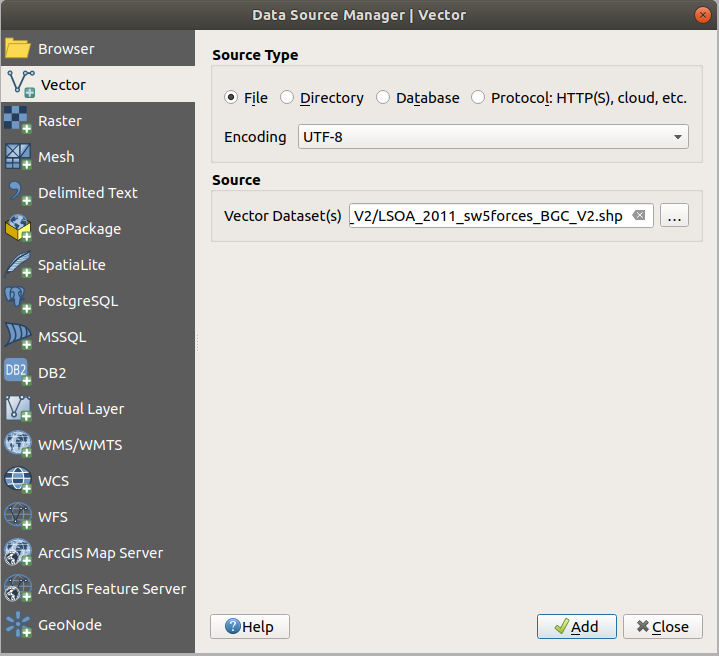
\includegraphics[width=\linewidth]{images/data_source_manager_window.png}
		\caption{Form to add a vector layer (shapefile)} \label{ft_fig_firstfig3}
	\end{subfigure}\hspace*{\fill}
	\begin{subfigure}{0.3\textwidth}
		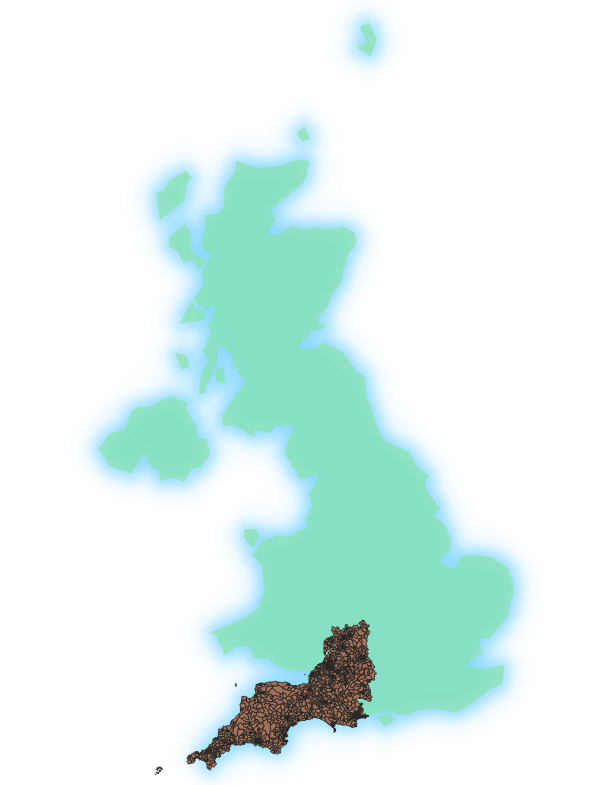
\includegraphics[width=\linewidth]{images/shapefile_added_to_uk_basemap.png}
		\caption{Shapefile containing LSOAs for SW England and UK basemap} \label{ft_fig_firstfig3}
	\end{subfigure}
\end{figure}

\textbf{Result}: The shapefile is displayed in the map canvas, the file is listed in the Layers panel, and (if you have it selected,) the Layers Styling panel is enabled.\\

From now on we will refer to this shapefile as a \textit{layer}.\\

Each open layer is listed in the \textit{Layers Panel}. The order they exist in this list determines the order that they are rendered on the map canvas.\\

Practice selecting and deselecting the layers open in your project (uk, point files and shapefile), and change the order they are rendered by dragging and dropping.

\null\newpage

\section{Attribute table}

As with all layers, this shapefile has an attribute table, layers property window, and can have it's symbology changed using the \textit{Layers Styling} panel.\\

Open the attribute table
\begin{tabular}{@{}c@{}}
\includegraphics[width=4ex]{images/attribute_table_icon.png}\end{tabular}. It only contains 4 fields. In this next few steps we will be adding fields into this shapefile from our own datafile. We will use the unique code in field "LSOA11CD" in oder to perform this join.

\section{Practice what you've learnt on this shapefile}

\begin{enumerate}
	\item 
	Move between selecting features on the map canvas (select feature tool), and identifying them in the attribute table (move selected rows to top of table)
	\item 
	Use Identify feature tool
	\item 
	Move between selecting features in the attribute table, and identifying them in the map canvas
	\begin{enumerate}
		\item 
		Select rows manually
		\item 
		Use select \& filter features form
		\item 
		Use select by expression
	\end{enumerate}
	\item 
	Save selected features as new feature layer
\end{enumerate}

%Task: Can you select the features for Exeter and save these as a new shapefile?

%Zoom to shapefile layer and deselect features
%\begin{tabular}{@{}c@{}}
\includegraphics[width=4ex]{images/deselect_features_icon.png}\end{tabular}. 